\documentclass[12pt]{report}
\usepackage[utf8]{inputenc}
\usepackage[french]{babel}
\usepackage[T1]{fontenc}
\usepackage{amsmath}
\usepackage{amsfonts}
\usepackage{amssymb}
\usepackage{graphicx}
\usepackage{titlesec}
\usepackage{caption}
\usepackage{titling}
\usepackage{booktabs}
\usepackage{enumitem}
\usepackage{eurosym}
\usepackage{epigraph}
\usepackage{hyperref}
\usepackage{fontspec}
\usepackage{ragged2e}
\usepackage{parskip}
\usepackage{wrapfig}
\usepackage{calc}
\usepackage{float}

\graphicspath{ {../../static/} {img/} }
\setlength{\droptitle}{-10em}
\titleformat{\chapter}[hang]{\normalfont\huge\bfseries}{\thechapter. }{0em}{}

\begin{document}

\title{
	{\vspace{3em}\protect\centering\protect
\includegraphics[width=0.9\textwidth]{Pacification_logo}}\\
	{\vspace{4em}\Huge Rapport de soutenance}\\
	{\large Brainless Devs}
}
\author{
	Thibault Allançon\\
	Valérian Fayt
	\and
	Antoine Gonzalez\\
	Cédric Parpet}
\date{
	{\vfill\protect\centering\protect
\includegraphics{brainless_devs.pdf}}\\
	Dossier Projet Informatique\\
	Info-Sup EPITA\\
	Mai 2018
}

\maketitle
\tableofcontents

\chapter{Introduction}

La deuxième phase de développement de \textit{Pacification} touche à sa fin.
Durant ces quelques semaines, nous avons pu beaucoup progresser sur l’évolution
du jeu, qui commence à réellement prendre forme. 

Nous somme partis d’un éditeur de map avec des fonctionnalités basiques pour
arriver à un solo et un multijoueur jouables, avec des unités capables
d'interagir avec leur environnement. Le réseau transmet correctement les
informations, la map dispose d’une génération procédurale et d’un brouillard de
guerre, et tous nos assets sont prêts.

Malgré l’apparition de nouvelles difficultés, tous les membres du groupe ont pu
travailler sur leurs parties et le résultat de cette période est conforme à nos
attentes.

Dans ce rapport, nous expliquerons avec plus de précision tout ce qui a été
réalisé durant cette phase, ainsi que ce qu’il reste à faire avant la
soutenance finale.

\begin{figure}
    \centering
    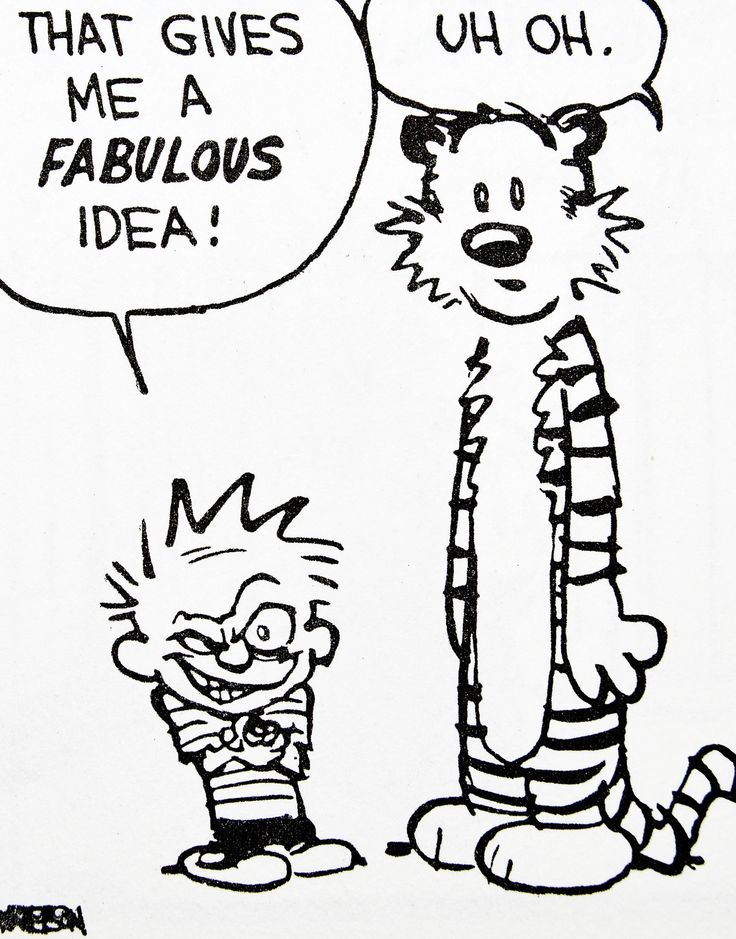
\includegraphics[width=0.6\textwidth]{project_mood_S2}
    \caption*{\textit{Calvin and Hobbes}, Bill Watterson}
\end{figure}

\chapter{Cahier des charges}

Cette fois-ci, pas de changement nécessaire sur la répartition des tâches.

\vspace{1cm}

\begin{center}
    \begin{tabular}{@{} l *4c @{}}
        \toprule
        \multicolumn{1}{c}{}    & \textbf{Soutenance 1}  & \textbf{Soutenance 2}  & \textbf{Soutenance 3} \\ 
        \midrule
        Map & 65\% & 100\% & 100\% \\
        IA & 30\% & 70\% & 100\% \\
        Réseau & 30\% & 75\% & 100\% \\
        Assets & 50\% & 100\% & 100\% \\
        Interface & 10\% & 80\% & 100\% \\
        Site & 10\% & 95\% & 100\% \\
        Gameplay & 40\% & 80\% & 100\% \\
        Budget pizza & 100\% & 60\% & null\\
        \midrule
        Jouabilité & 25\% & 60\% & 100\% \\
        \bottomrule
    \end{tabular}
\end{center}

\vspace{0.5cm}

Les assets étant finalement terminés, l’interface - actuellement en retard,
plutôt 70\% que 80\% - pourra avancer rapidement et être terminée sous peu.

Le site web n’a pas réellement eu besoin d’être amélioré depuis la première
soutenance car il était en avance. Une mise à jour des informations était
cependant nécessaire pour informer de notre avancement, et changer les images du
jeu qui a bien évolué depuis.

Les dernières fonctionnalités de la map sont désormais en place, c'est-à-dire la
génération automatique de carte, le brouillard de guerre ainsi que les unités
qui peuvent se déplacer et intéragir avec la map. Il restera toujours quelques
légers peaufinements pour la soutenance finale.

L’IA a progressé comme prévue, son fonctionnement sera détaillé plus bas.

Le gameplay a également atteint ses objectifs, les unités sont implémentées et
fonctionnelles, les villes sont utilisables, le Player fait partie intégrante
du jeu, il ne reste maintenant qu’à implémenter une économie au jeu grâce aux
ressources et aux bâtiments des villes ; et à prendre les biomes en compte dans
les calculs des unités.

\chapter{Avancement}

\section{Map (Thibault)}

La première chose qu'il a fallu intégrer à la map était les unités en elles
mêmes. Le système de pathfinding était déjà en place, mais le fait de
positionner les unités, de pouvoir les sélectionner, les déplacer, représentait
une tâche importante et majeure du jeu. 

En utilisant des courbes de Bézier nous avons désormais des déplacements fluides
et assez naturels sur la carte, d'autant plus que ces courbes nous permettent de
gérer facilement l'orientation des unités qui se tournent avant et pendant leurs
déplacements.

Lors de la soutenance précédente nous avions mis en place des menus pour éditer
la carte afin de montrer les différentes fonctionnalités. Nous avons décidé de
réutiliser cette partie pour mettre en place un éditeur de map afin de créer ses
propres cartes sur lesquelles on pourra ensuite jouer.

\begin{figure}[H]
    \centering
    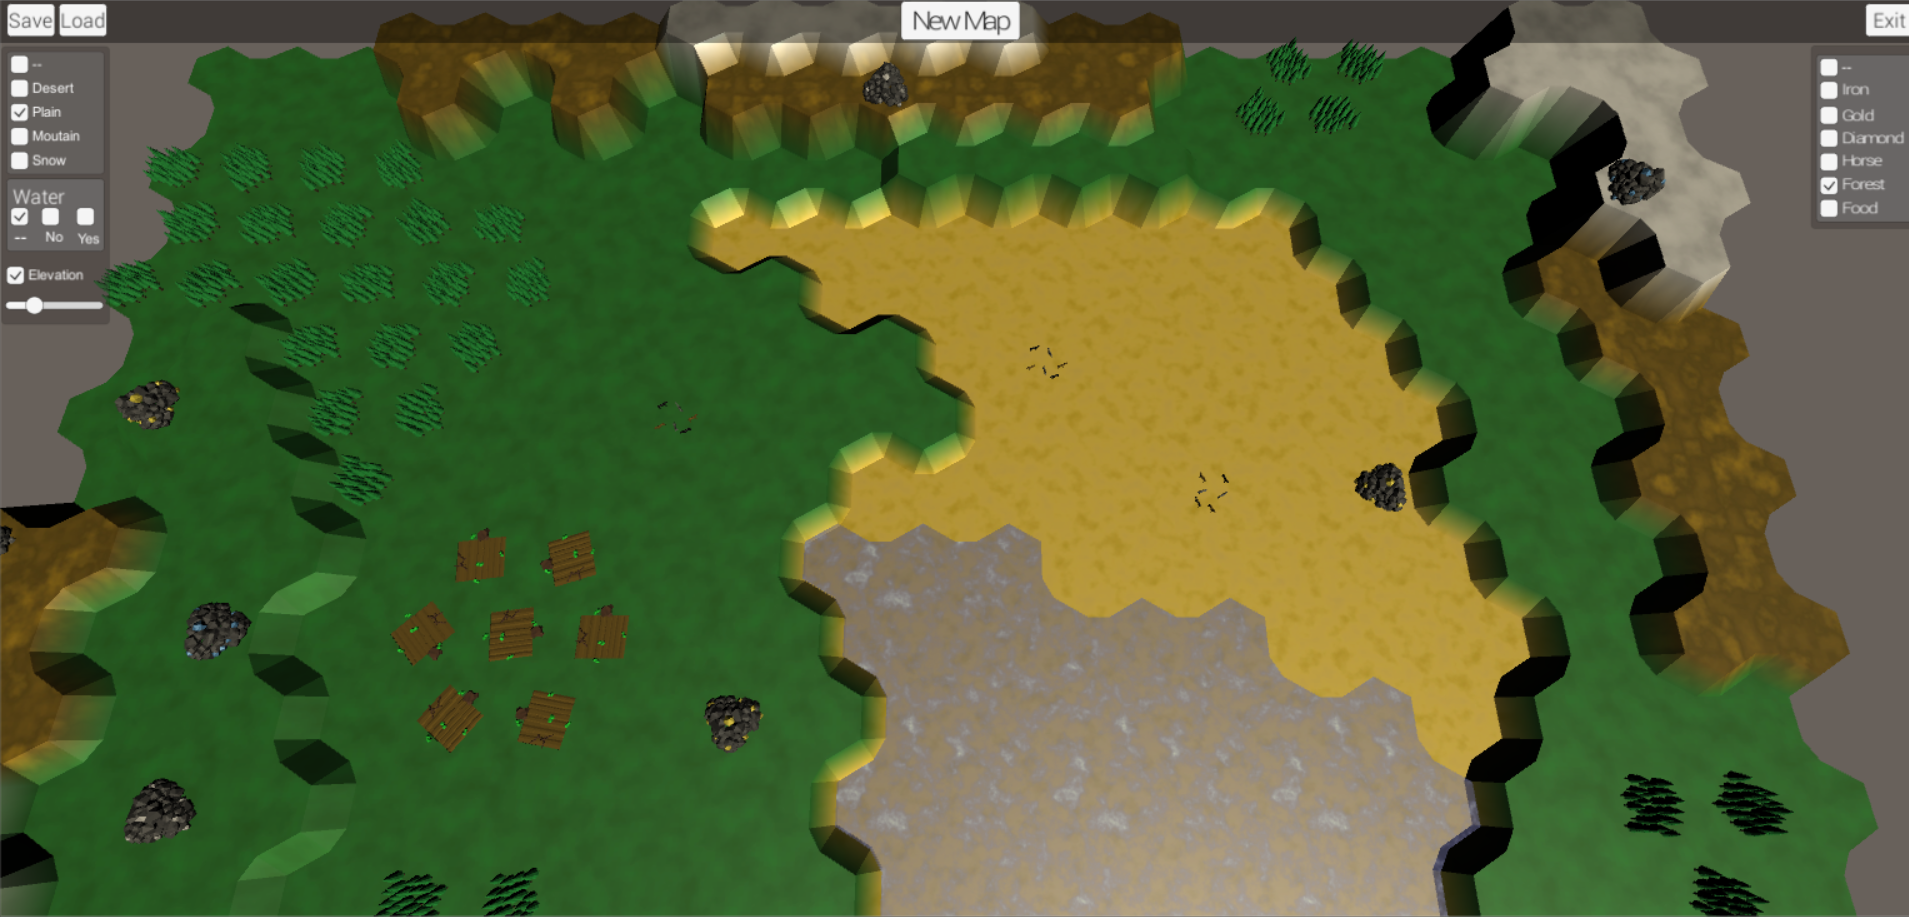
\includegraphics[width=0.8\textwidth]{EditorScreen}
    \caption{Editeur de map}
\end{figure}

Cependant, il était prévu depuis le début de générer des cartes lors d'un début
de partie pour avoir à chaque nouveau lancement de jeu une situation différente.

Une génération de carte procédurale est désormais intégrée au jeu, et le joueur
peut maintenant sélectionner s'il souhaite utiliser une carte qu'il a lui même
édité ou bien en générer une nouvelle. Cette génération utilise une dizaine de
paramètres que l'on peut configurer afin d'obtenir des types de cartes très
variés : pourcentage de terre, taille des régions, nombres de régions, élévation
maximale des montagnes, érosion des terrains, etc. Pour construire une nouvelle
carte il faut déterminer les bouts de terres que l'on veut surélever (de base,
tout le terrain est submergé par l'eau). De l'aléatoire est donc nécessaire pour
choisir cet emplacement, il suffit ensuite de rester dans les alentours de cette
case à l'aide d'un parcours en largeur. Une fois le terrain formé, on attribue
le type du biome en fonction de l'élévation (désert et plaine pour les terrains
les plus plats, montagnes et neige pour les terrains extrêmes).

\begin{figure}[H]
    \centering
    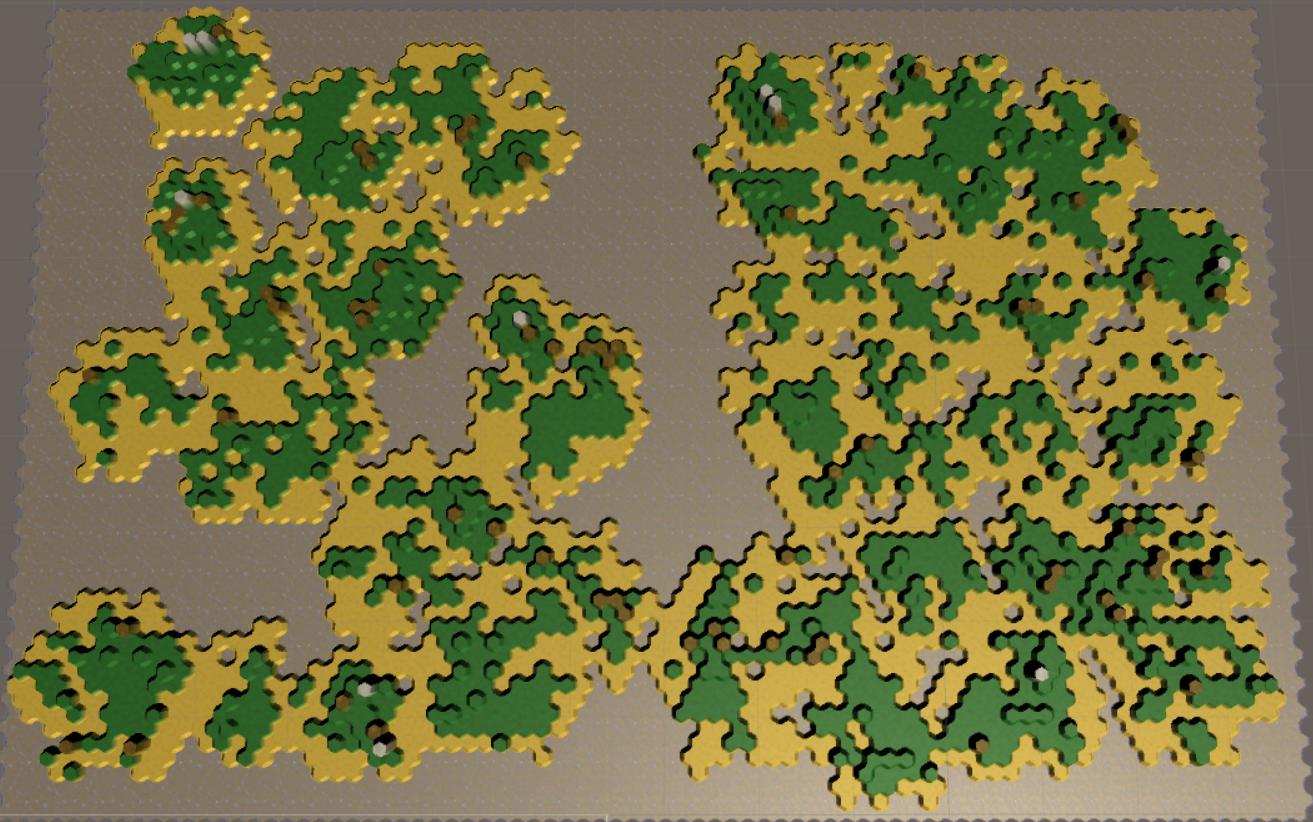
\includegraphics[width=0.8\textwidth]{MapGen1}
    \caption{Génération de carte 1}
\end{figure}

\begin{figure}[H]
    \centering
    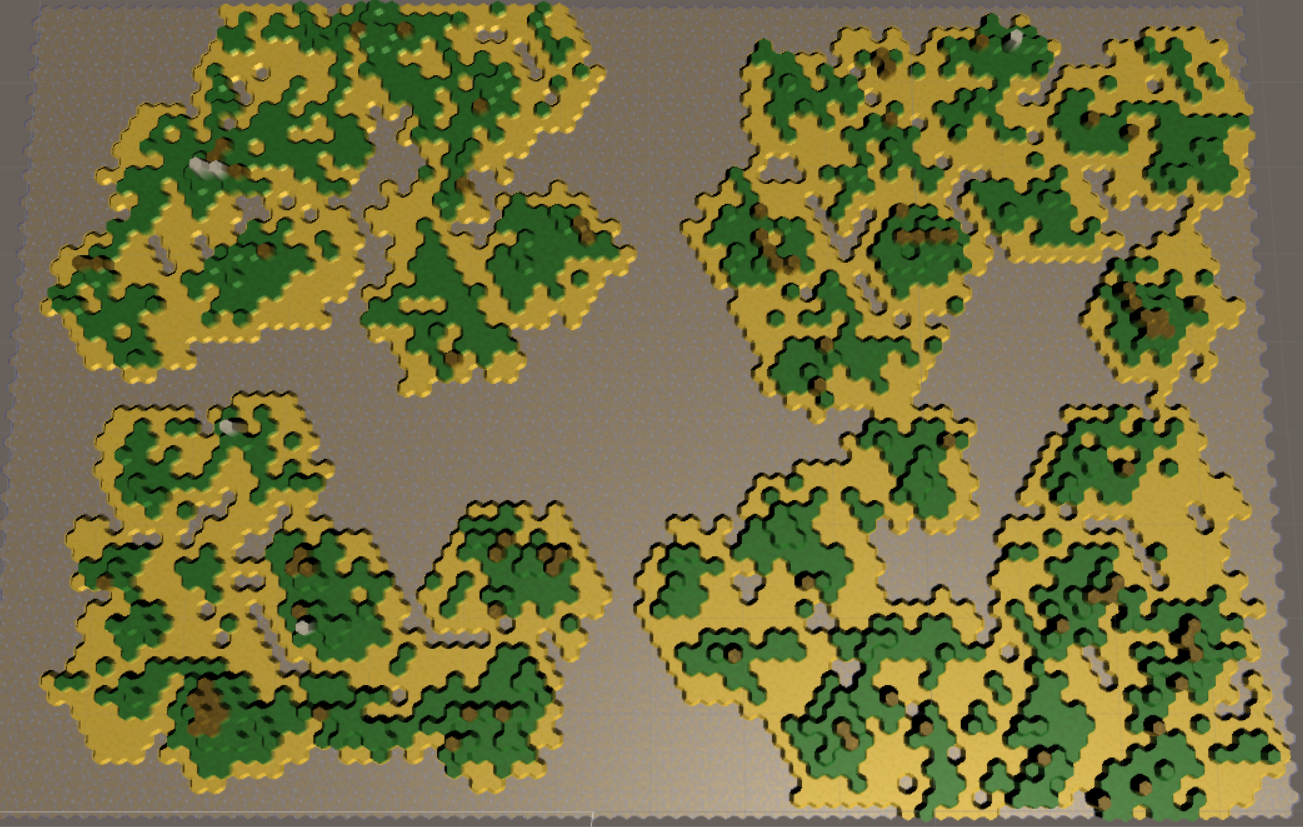
\includegraphics[width=0.8\textwidth]{MapGen2}
    \caption{Génération de carte 2}
\end{figure}

La dernière fonctionnalité que nous voulions intégrer à la carte de Pacification
était le brouillard de guerre, élément indispensable pour ce type de jeu de
stratégie. Il a fallu adapter les shaders ainsi que les textures pour cacher ou
montrer des parties de la carte en fonction de plusieurs critères comme : la
hauteur de la case sur laquelle se trouve l'unité, son nombre de point de
vision, si la case a déjà été visité ou non. On différencie donc deux types de
brouillard : d'une part les terrains inexplorés qui sont totalement cachés du
joueur et de l'autre les terrain précédemments explorés mais hors de vision et
portée de l'unité.

\begin{figure}[H]
    \centering
    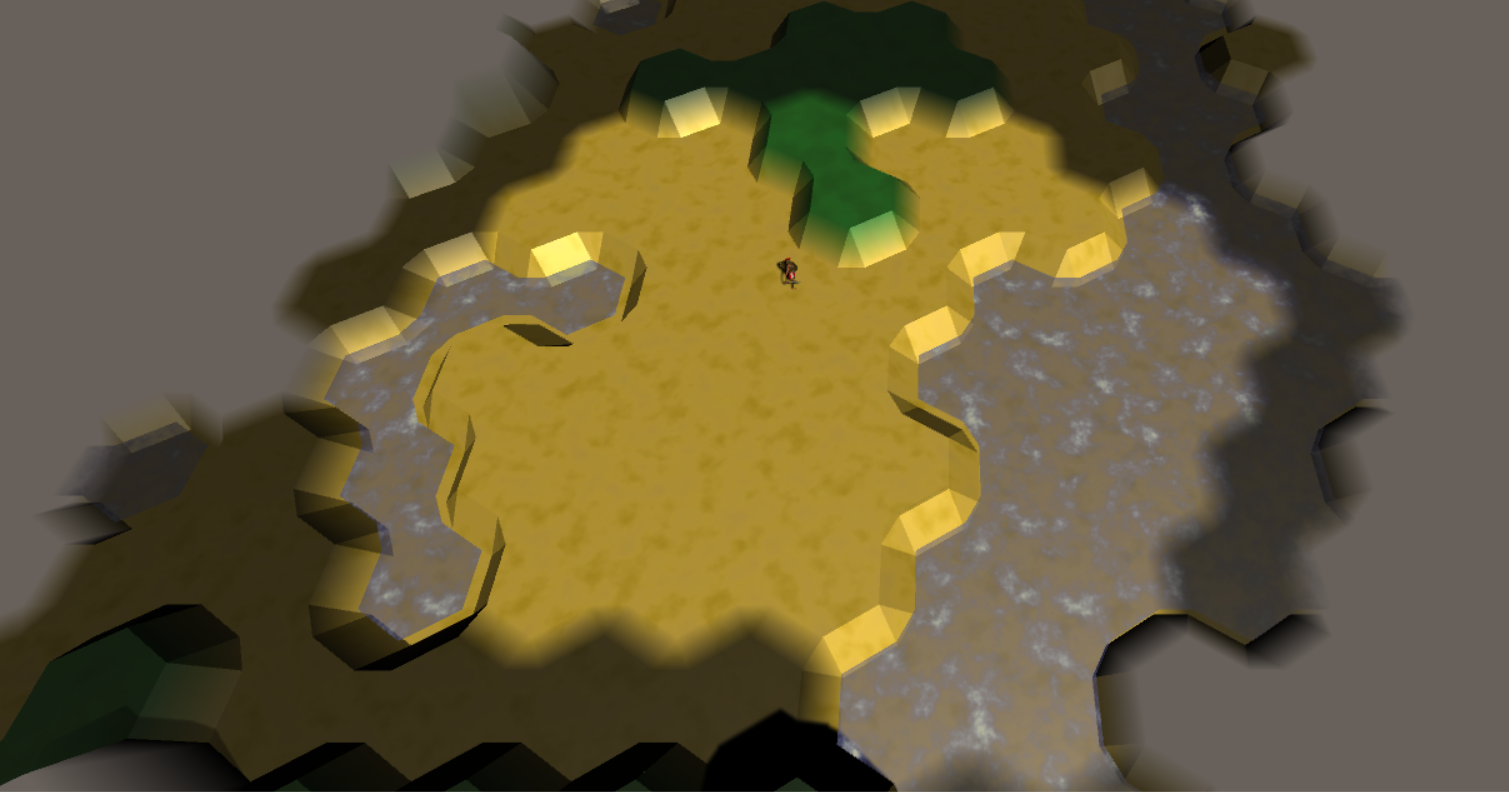
\includegraphics[width=0.8\textwidth]{FogOfWar}
    \caption{Brouillard de guerre}
\end{figure}

\section{Réseau et multijoueur (Valérian)}

Les bases du réseau ayant été mises en place pour la première soutenance, les
objectifs pour celle-ci consistaient majoritairement à adapter les nouvelles
fonctionnalités apportées par le gameplay ainsi que par l’avancé de la map et
de l’IA, mais aussi à implémenter des choses nouvelles tel qu’un tchat et le
principe de tour par tour, sur lequel se base le jeu.

Concernant le gameplay, il a fallu prendre en compte l’implémentation des
différentes unités ainsi que des villes. La difficulté qui s’est présentée à
été de devoir synchroniser tous ces éléments, en gardant les liens
d'appartenance de chaque unité. Il a donc été nécessaire de recréer chez tous
les clients, une copie minimale des autres joueurs. Ainsi, chacun possède une
liste des autres joueurs présents, permettant d'identifier facilement
l'appartenance des unités, et des villes sur la map.

Pour la map, l’objectif était de transmettre en début de partie une carte de
jeu généré aléatoirement. Cela nécessitant de réduire la map au strict minimum
pour ensuite l’envoyer sous forme de string via le système Serveur/Client
construit pour la première soutenance. Pour cela, nous avons utilisé le système
de sauvegarde qui permet d’enregistrer la carte sous une forme condensée.
Réaliser cet objectif n’a pas été une difficulté en soit mais nous a permi de
nous rendre compte de certaines limites de vitesses de notre système réseau,
lors des transferts de cartes de taille importante.

Du côté de l’IA, il a fallu adapter la gestion du tour par tour sur lequel nous
reviendrons prochainement, afin d'avoir un joueur machine dans la partie.

S'intégrant parfaitement dans un jeu de stratégie où des alliances peuvent
retourner la partie, nous avons décidé d’ajouter un tchat pour “pimenter la
partie”. Le tchat comprend en effet plusieurs fonctions utiles tel que les
messages globaux, permettant de communiquer avec tous les autres joueurs, mais
aussi des messages privés pour ne partager ses stratégies qu’avec les joueurs
que vous souhaitez.

L’implémentation du tchat à ouvert la porte à l’implémentation d’une console de
débogage pour nous faciliter les phases de test durant le développement de
nouvelles fonctionnalitées. On compte dans cette console les commandes
suivantes : 

/help : Commande qui suivi d’une autre, permet d’obtenir la documentation
nécessaire au fonctionnement de cette dernière.

/kick : Commande permettant d’éjecter un joueur de la partie en cas de
nécessité, en dehors de l'Hôte de la partie.

/clear : Commande permettant de nettoyer de l’écran soit tous les messages du
tchat (clear msg) ou les unités présentes sur la map (clear unit).

/fog : Commande permettant d’activer ou désactiver le brouillard de guerre.

/code :  Commande permettant d'accéder à des actions peu légitimes lors d’une
vraie partie, mais pouvant donner un coup de boost si vous êtes dans le besoin.

Finalement, la dernière fonctionnalité mise en place à été le tour par tour,
principe même du jeu. Il s’agissait pour cette tâche de lier à la fois le
gameplay (en empêchant les joueurs de jouer si ce n’est pas leur tour),
l’interface (en affichant différents éléments en fonction de la possibilité du
joueur à bouger où non), et finalement le réseau (en évitant que plusieurs
joueurs puisse jouer en même temps).

\section{Gameplay (Antoine, Thibault)}

Le gameplay a bien avancé. Nous disposons à présent d’unités correctement
implémentées.

Au début de la partie, le joueur commence avec un colon et un fantassin. Le
colon permet de construire la première ville du joueur, tandis que l’unité
offensive peut permettre d’explorer les alentours et de découvrir la carte,
alors recouverte par le brouillard de guerre. 

\begin{figure}[H]
    \centering
    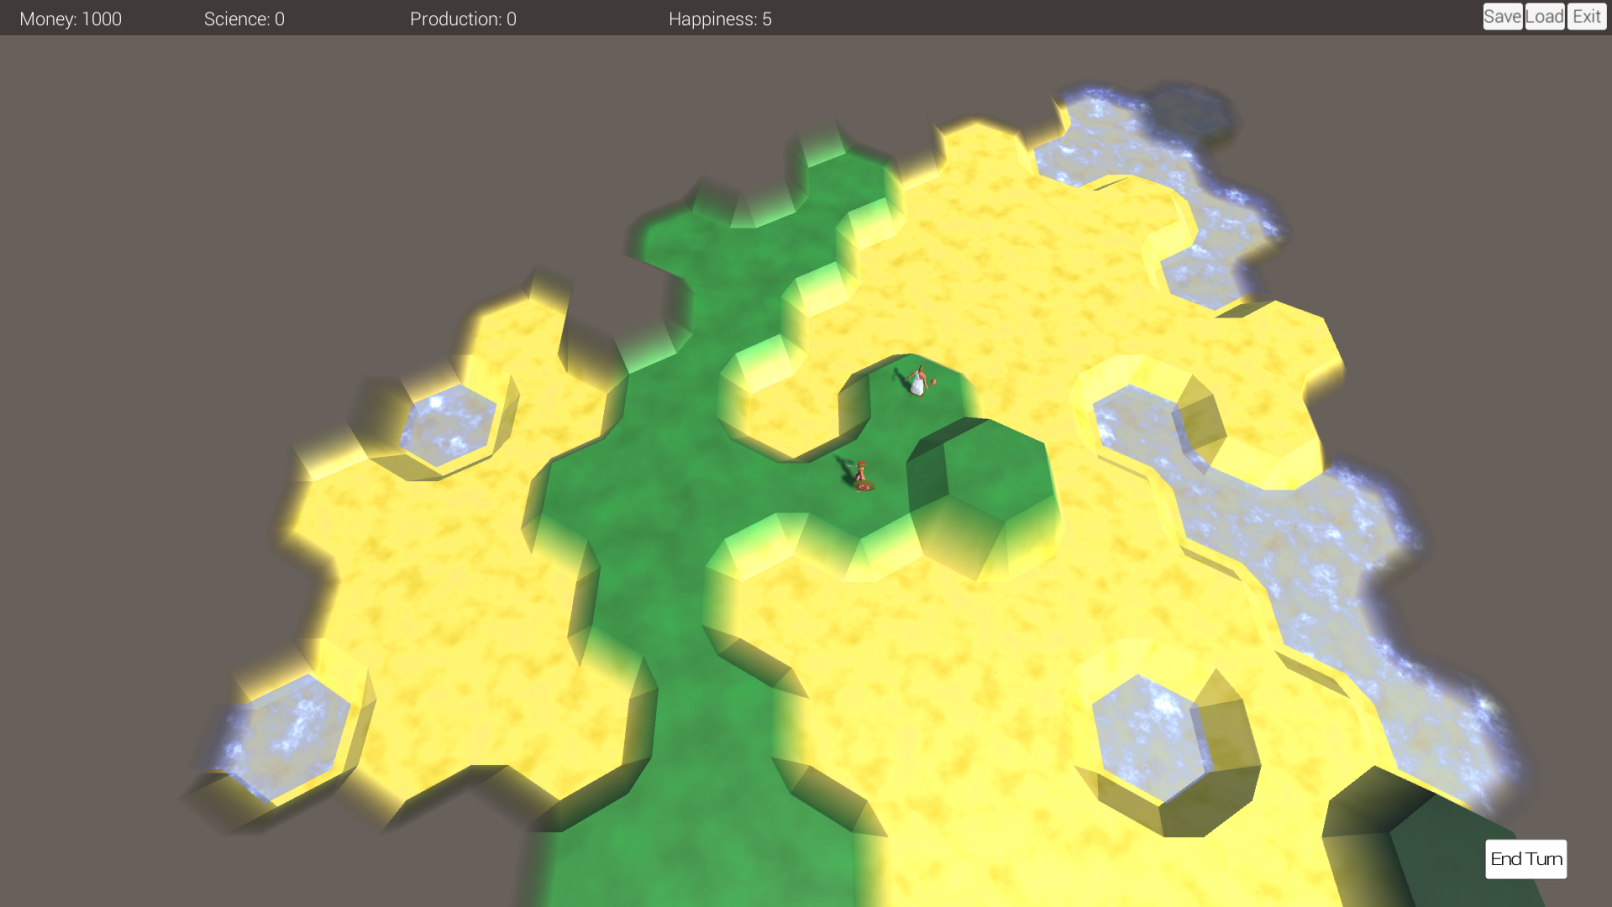
\includegraphics[width=0.8\textwidth]{InitialSituation}
    \caption{Situation initiale}
\end{figure}

Les unités peuvent donc se déplacer et activer leur action propre (construire
une ville pour le colon, exploiter une ressource pour l'ouvrier, attaquer un 
ennemie pour les unités offensives).

\begin{figure}[H]
    \centering
    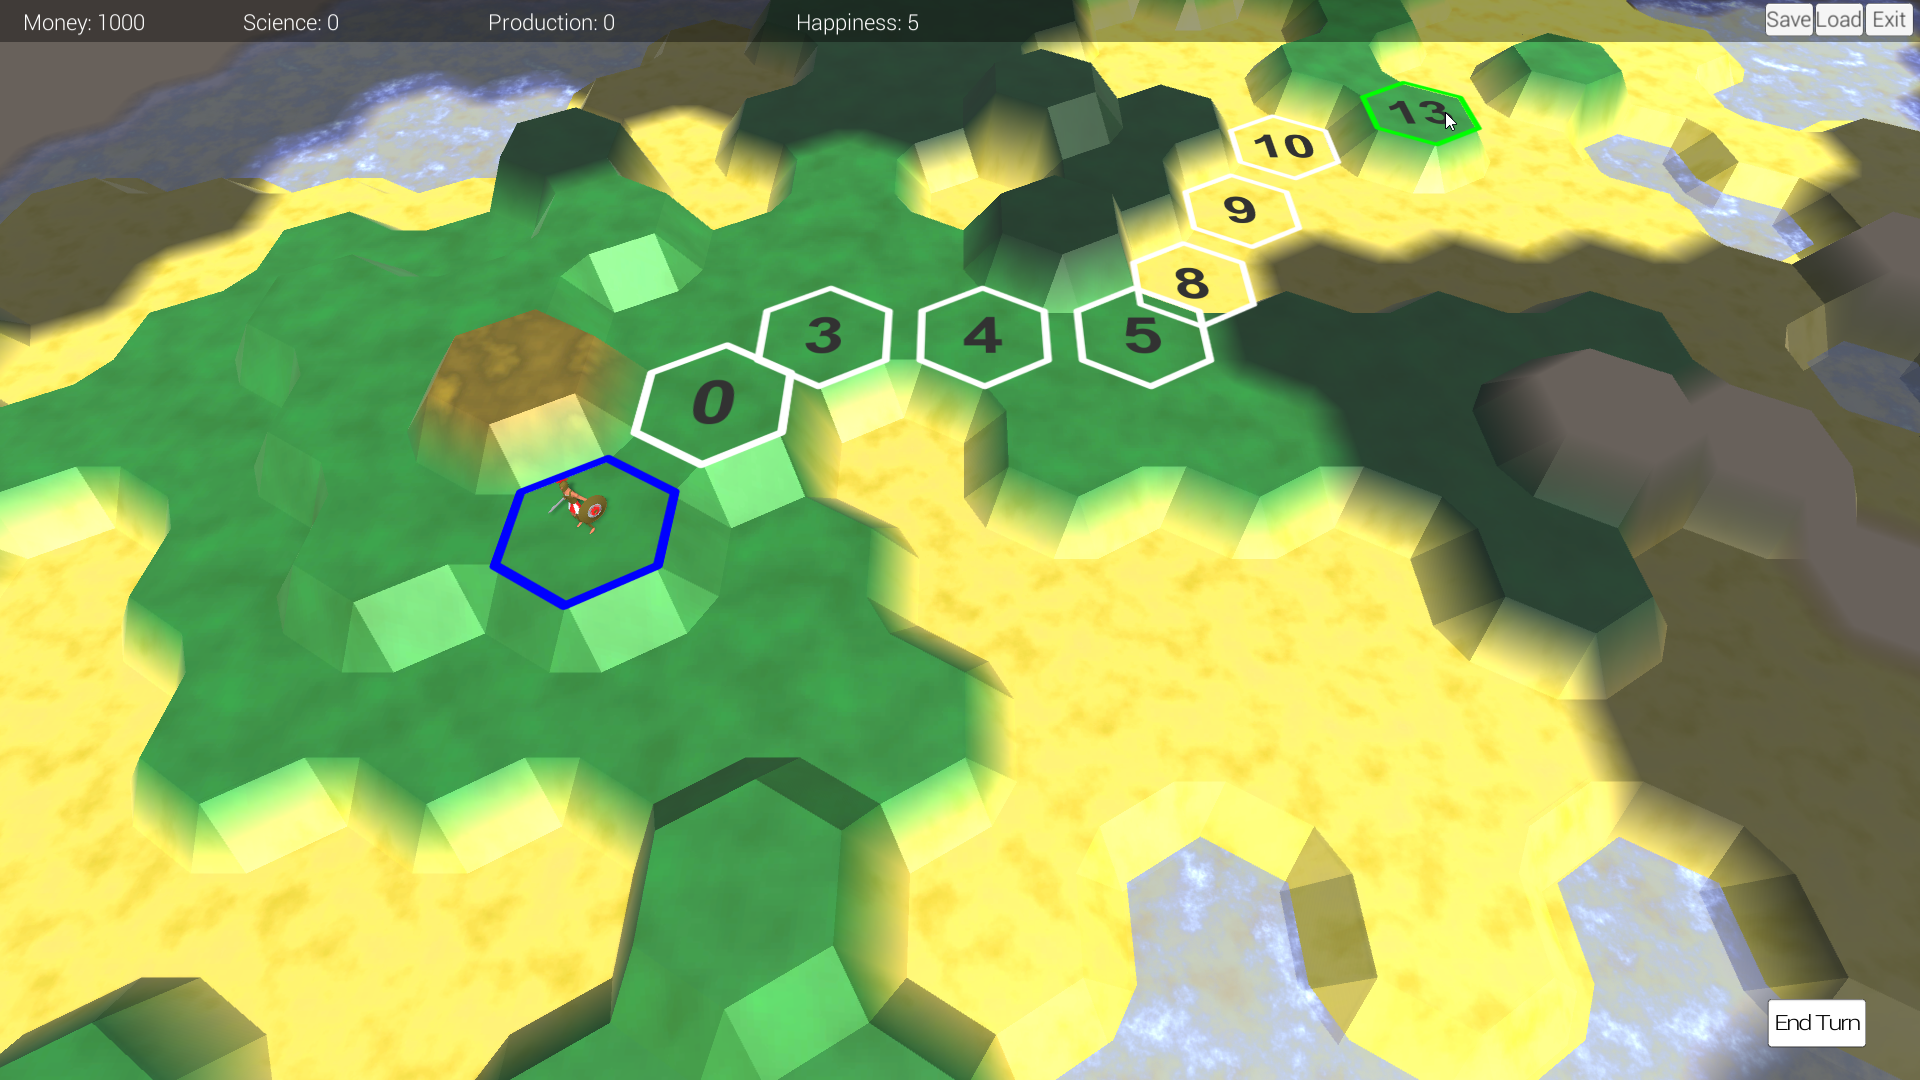
\includegraphics[width=0.8\textwidth]{Pathfinding}
    \caption{Pathfinding}
\end{figure}

La ville permet pour le moment de produire d’autres unités qui apparaîtront dans
dans cette dernière grâce au menu “barrack”. Il est ainsi possible de créer un
autre colon, un travailleur, ou une des différentes unités offensives.

Chaque unité possède des caractéristiques qui lui sont propres, ainsi qu’un
modèle 3D assigné à sa création selon son type (les unités d’attaque possèdent
un second modèle amélioré qu’elles obtiennent à partir du niveau 11). Ces
statistiques, présentées dans les tableaux de la première soutenance, influeront
notamment sur le nombre de tour nécessaire pour tuer une cible et  la vitesse de
déplacement.

La ville disposera également d’améliorations, cependant elles dépendent de la
population ainsi que de l’économie qui seront implémentés lors de la dernière
phase de développement.

\section{Assets (Cédric)}

Les assets ont été finis à 100\%, les modèles 3D sont basés, pour la plupart,
sur mes premières créations pour faire les suivantes. Trois nouvelles textures
ont été créées spécialement pour les villes.

\begin{figure}[H]
    \centering
    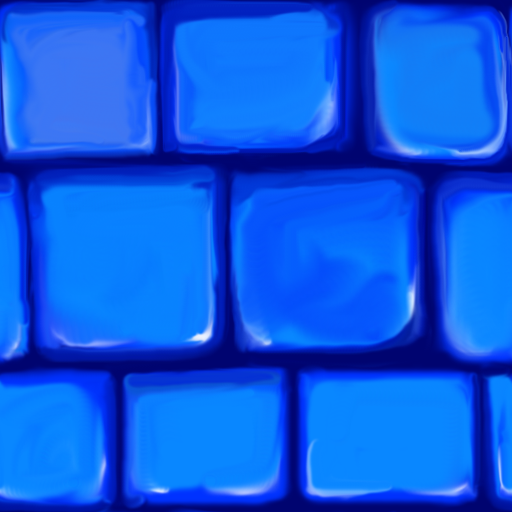
\includegraphics[width=0.3\textwidth]{BlueRoof}
    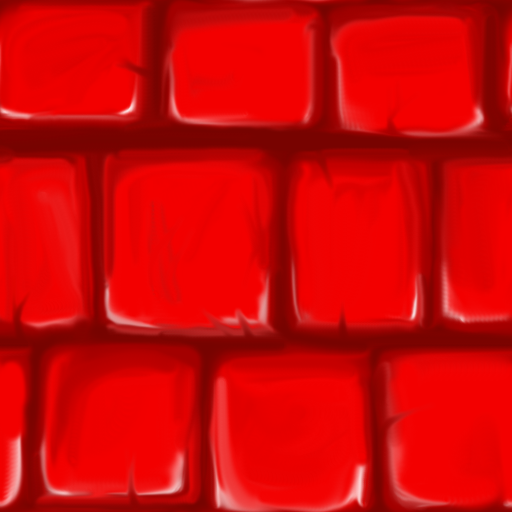
\includegraphics[width=0.3\textwidth]{RedRoof}
    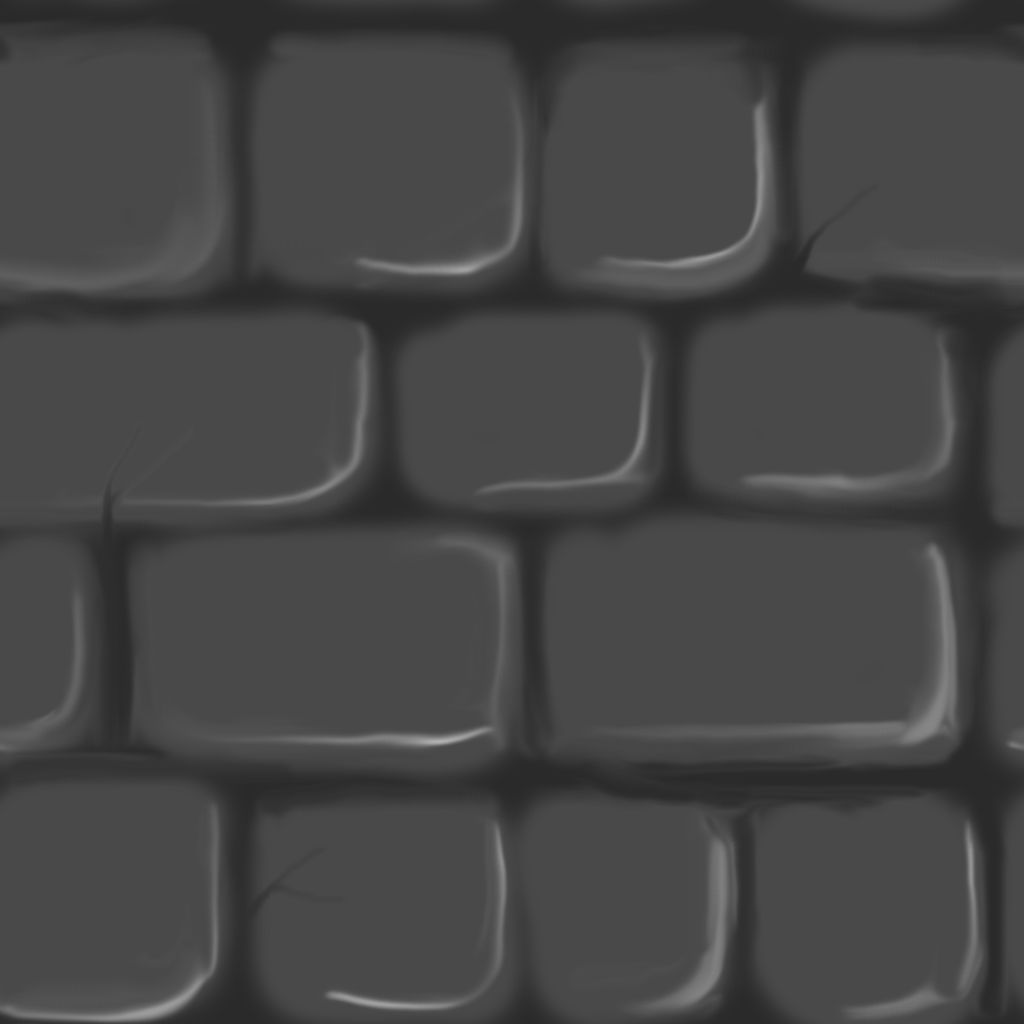
\includegraphics[width=0.3\textwidth]{DarkStoneWall}
    \caption{BlueRoof, RedRoof, DarkStoneWall}
\end{figure}

Les modèles 3D des bâtiments sont tous finis. Seuls les villes ont nécessité de
nouveaux modèles car ceux de la dernière soutenance ont pu être réutilisé, comme
prévu, pour gagner du temps. Il existe deux modèles différents pour les
ressources du jeu : la version naturelle et la version exploitée.

\begin{figure}[H]
    \centering
    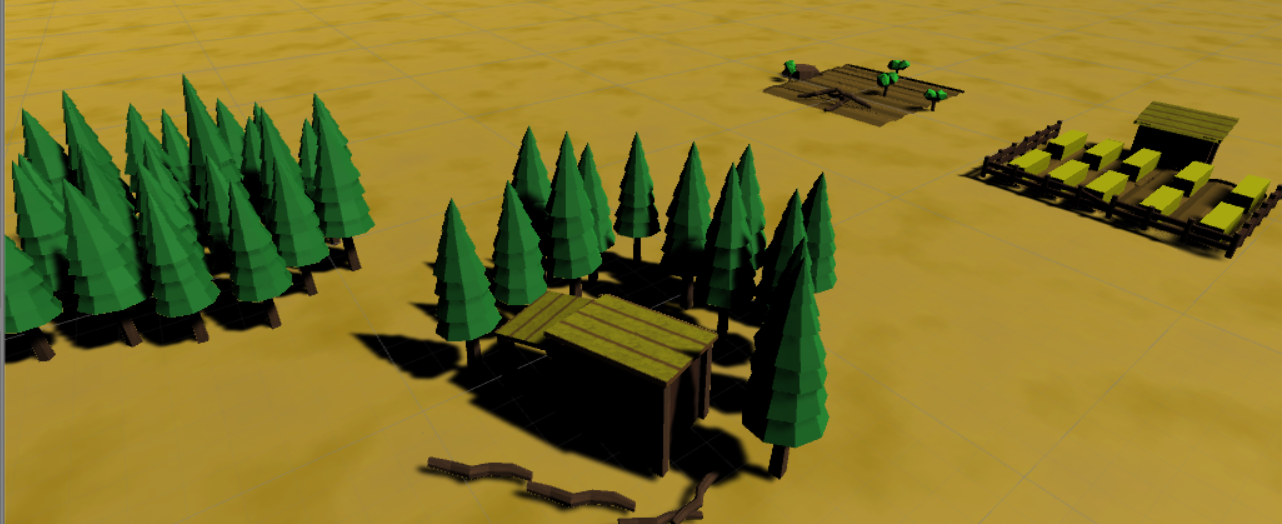
\includegraphics[width=0.8\textwidth]{assets_food_forest}
    \caption{Version naturelle et exploitée}
\end{figure}

\begin{figure}[H]
    \centering
    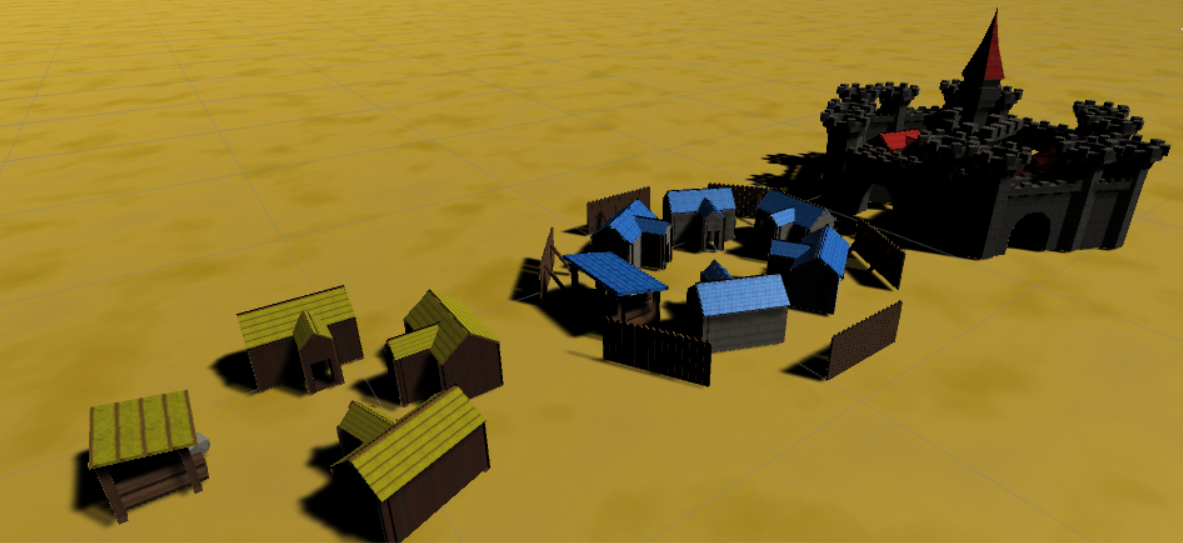
\includegraphics[width=0.8\textwidth]{AllCitiesScreen}
    \caption{Les différents modèles de ville}
\end{figure}

Concernant les unités ajoutées il y a les deux versions d’unité à portée, les
deux versions des unités de siège (catapulte et canon), et le cavalier qui
correspond à l’amélioration de l’infanterie. Comme pour les modèles précédent,
la création des unités (notamment le canon et la catapulte) se sont fait à
l’aide d’image de référence. Les modèles des unités humaines ont été construits
à partir du modèle humain de base créer durant la première période du projet.

\begin{figure}[H]
    \centering
    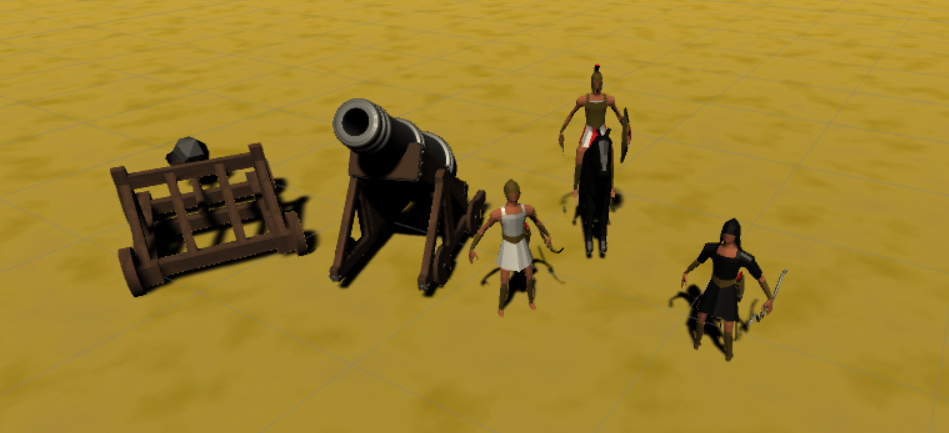
\includegraphics[width=0.8\textwidth]{NewUnits}
    \caption{Nouvelles unités}
\end{figure}

Les animations des personnages ont toujours été considéré comme du bonus.
Cependant, des premiers tests pour la catapulte ont été faits, mais ne sont pas
encore intégrés au jeu. Ces animations pourront être réutilisées par la suite
par le canon ou d'autres unités. L'animation des armatures humaines semblent
assez complexe à gérer, d'où l'utilisation d'un outil externe hébergé par le
site internet gratuit mixamo.com permettant de donner simplement une armature à
un personnage avec des animations fluides.

\begin{figure}[H]
    \centering
    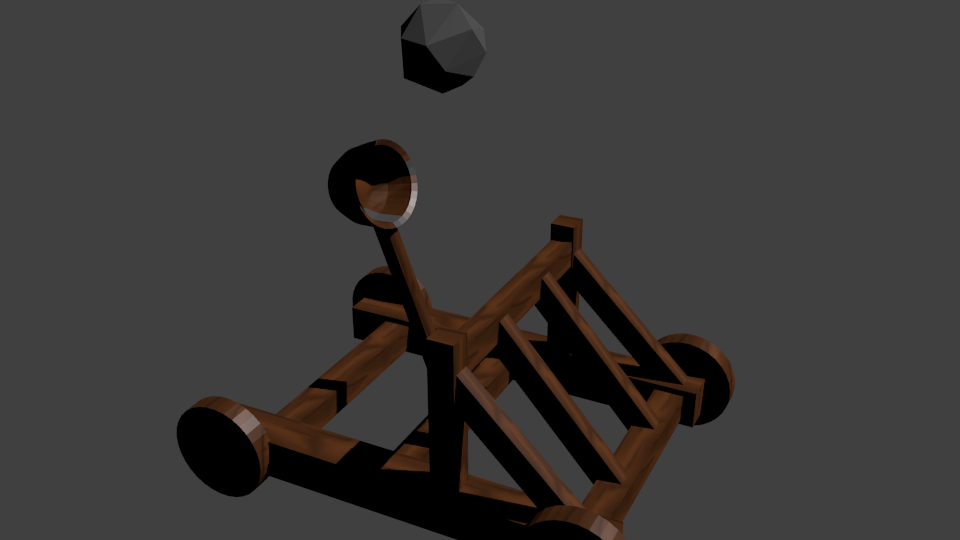
\includegraphics[width=0.8\textwidth]{CatapulteAnimation}
    \caption{Début d'animation}
\end{figure}

\section{Interface (Cédric, Valérian, Antoine)}

Pour le menu principal nous avons récupéré un asset créé par \textit{Michsky}
qui l’a rendu accessible à tous gratuitement sur internet. Le fait de
réutiliser un menu existant nous a permis de nous concentrer sur d'autres
aspects graphiques du jeu nécessitant une réelle customisation pour suivre le
thème de \textit{Pacification}. Le menu principal a donc été mis en place et
adapté rapidement au jeu :

\begin{figure}[H]
    \centering
    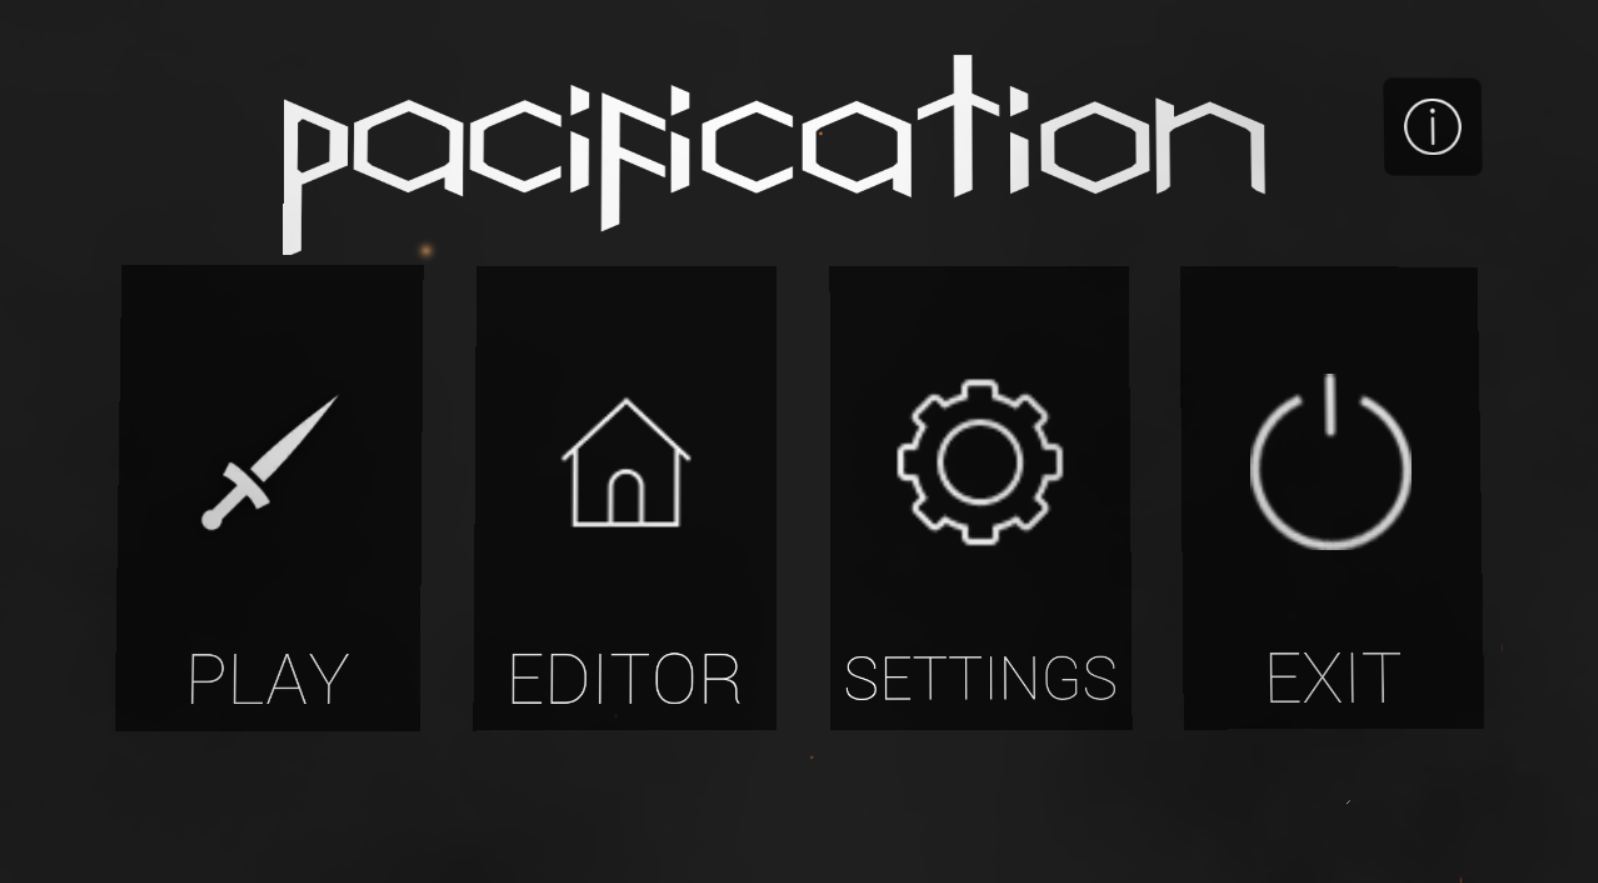
\includegraphics[width=0.8\textwidth]{MainMenuScreen}
    \caption{Menu principal}
\end{figure}

Le menu principal comporte un accès au “menu Play” qui regroupe les
fonctionnalités de jeu en solo et en multijoueur.

\begin{figure}[H]
    \centering
    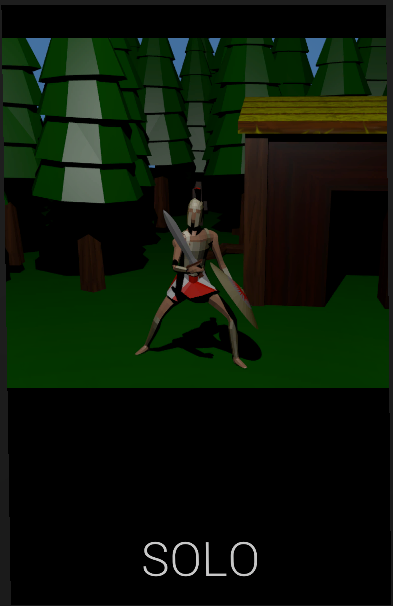
\includegraphics[width=0.3\textwidth]{SoloIcon}
    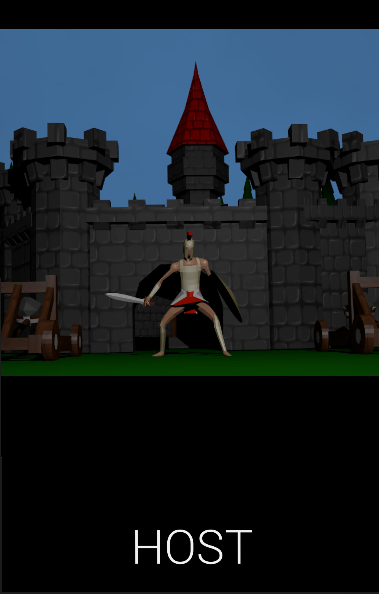
\includegraphics[width=0.3\textwidth]{HostIcon}
    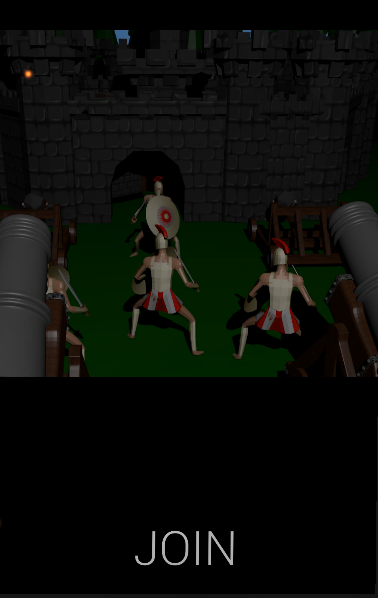
\includegraphics[width=0.3\textwidth]{JoinIcon}
    \caption{Menu Play}
\end{figure}

Les images apparaissant sur les boutons “Solo” “Host” et “Join” ont été faites
grâce à blender. Les positions du soldat ont été possible grâce à l’armature et
aux animations importés sur le site mixamo.com cité prècedemment. Un menu
“Paramètres” a été créé où l’on pourra par exemple gérer le son, la musique, et
les touches de jeu. Un bouton “informations” est disponible et mène aux crédits
du jeu. On navigue de menu en menu grâce à des déplacements de caméras qui
nous amènent sur des nouveaux canvas et des boutons back ont été placé pour
simplifier cette navigation.

Concernant l'interface dans le jeu, la sélection d'une ville déclenche
l'interface de la caserne (barrack) permettant de construire des unités. Un
bandeau d'information est désormais situé en haut de l'écran et informe le
joueur des informations de son empire (argent, productivité, science, bonheur
de la population). Dans l'éditeur de map ce bandeau est remplacé par de simples
bouttons permettant de sauvegarder, charger et générer une carte.

Enfin, un tchat est disponible pour s'envoyer des messages ou utiliser des
commandes spéciales. Son développement a représenté un certain challenge vis à
vis de l'interface, mais représente un élément important notamment pour
l'aspect multijoueur.

Une première musique d'ambiance a été rajouté dans le jeu en solo et en
multijoueur. On retrouve aussi différents effets sonores basiques comme les
sons de notification du tchat, ou l'apparition d'une tribu barbare dans les
environs.

\section{IA (Thibault)}

La partie réflexion sur l'IA lors de la première soutenance a permis une
implémentation rapide des tribus barbares. Le niveau de difficulté (facile,
normal, difficile) influe sur la fréquence d'apparition des unités barbares,
leurs nombres, ainsi que leurs niveaux par rapport à celui du joueur. Un son de
notification prévient de l'apparition d'une tribu barbare dans les environs.
L'IA pour l'instant se contente de créer les nouvelles unités adaptées autour
d'une ville du joueur (dans un certain rayon), il faudra donc ensuite réutiliser
les fonctionnalités de pathfinding pour que ces unités se dirigent et attaquent
la ville.

\section{Site Web (Valérian)}

En ce qui concerne le site web, des mises à jour de fonctionnalités n’ont pas
été nécessaire, car le site avait été développé avec de l’avance pour la
première soutenance. Il suffisait donc pour cette soutenance de le tenir à
jour, en ajoutant les articles correspondantes et les images de développement.

Cette soutenance a aussi été l’occasion de changer d'hébergeur, passant de Git
Pages à Lixia. Ce choix s’est principalement fait pour utiliser du PHP sur le
site, ainsi qu'avoir un nom de domaine gratuit plus court :
\url{pacification.lxa.li}.

\chapter{Avances, retards, difficultés rencontrées}

\section*{Map}

Les objectifs de la map sont tous remplis, terminant ainsi cette partie du jeu.
Le résultat du brouillard de guerre ainsi que du générateur de carte est très
satisfaisant, et rajoute réellement une nouvelle dimension au jeu. Les shaders
ont été difficile à correctement mettre en place afin d'avoir d'une part les
terres inexplorées et d'autre part les parties précédemment explorées mais hors
de vision des unités. La génération de map fut assez rapide à implémenter grâce
aux fonctions de la première soutenance pour modifier une carte. Les unités
peuvent maintenant se déplacer, s'orienter ainsi qu'intéragir avec leur
environnement.

\section*{Réseau et Multijoueur}

L’avancement du réseau a suivi le cours de son développement prévu, et continue
à prendre de l'avance. Tous les objectifs qui avaient été fixé pour cette
seconde soutenance sont donc réalisés avec le bonus du tchat. Il était question
de suivre les avancées du gameplay notamment l'implémentation des unités et
villes en réseau, mais aussi l'IA pour le mode solo. Le système de tour par tour
est maintenant en place, et la map est transmise en début de partie à tous les
clients.

Une fois les objectifs remplis, un tchat a pu être mis en place pour discuter
dans le mode multijoueur ou encore utiliser des commandes de triche.

\section*{Gameplay}

Si on reprend la hiérarchie des classes présentée lors de la première
soutenance, on peut voir que les unités sont complètement implémentées, et les
villes le sont en partie (l’économie reste à faire). Le “Player” est également
géré par le réseau et permet de coordonner les villes et les unités.  Les biomes
sont présents dans le code, mais pour le moment ils ne sont pas pris en compte
par le pathfinding et la génération de la map car il reste à organiser une
probabilité d’apparition des différentes ressources.

\begin{figure}[H]
    \centering
    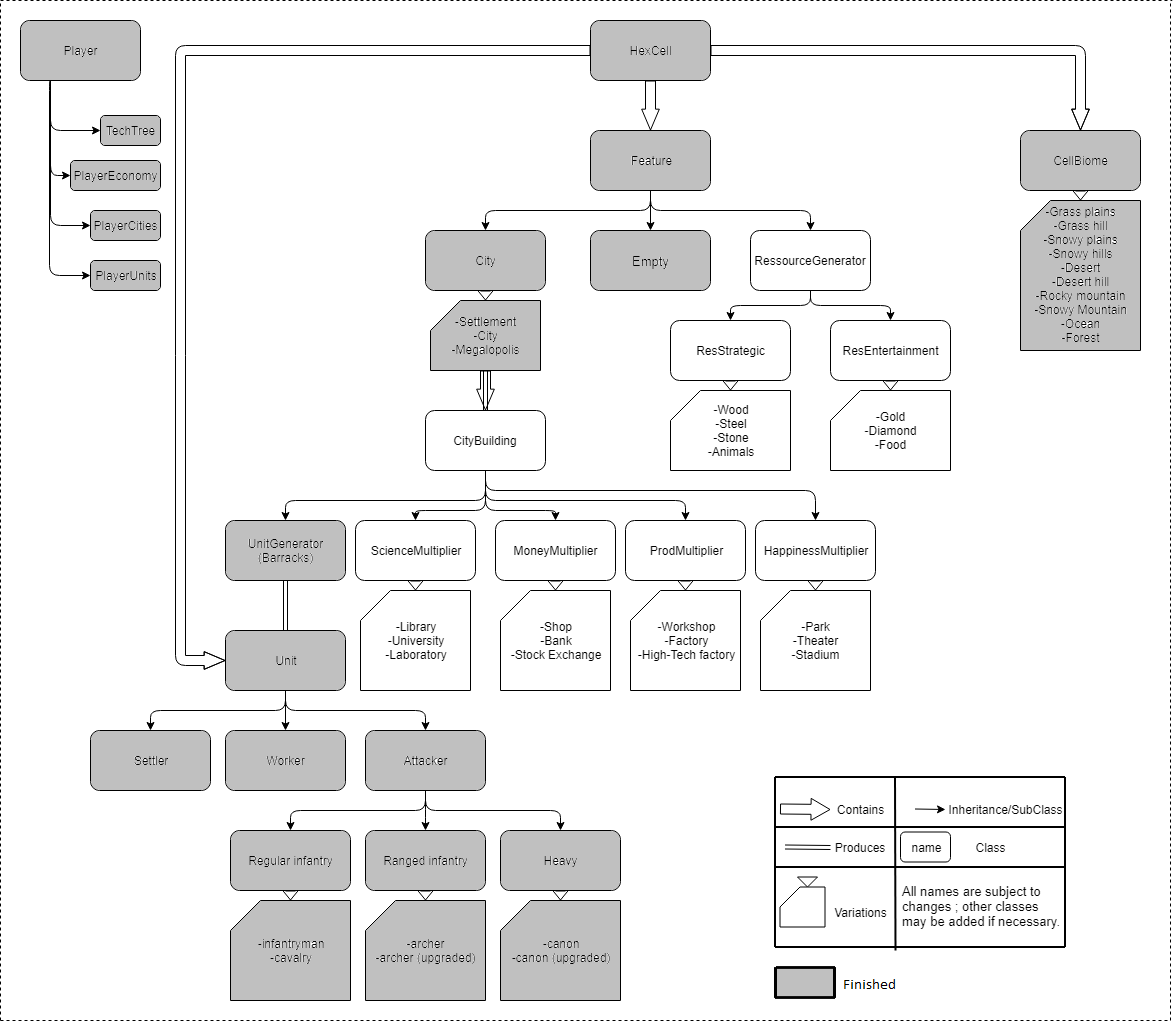
\includegraphics[width=1\textwidth]{class_hierarchy}
    \caption{Hiérarchie (avancement)}
\end{figure}

La difficulté principale durant cette période a été d'apprendre à "lier" les
classes selon Unity (qui doivent être instanciées pour être affichées sur la
map), et celles de C\# qui appellent un constructeur (dont j'avais besoin pour
gérer les unités et les villes), sans pour autant créer de conflits avec les
autres systèmes eux aussi nécessaires au fonctionnement du jeu. Cela m'a pris
plus de temps que prévu et a été une source de stress, mais tout a fini par
fonctionner.

\section*{Assets}

\section*{Interface}

\section*{IA}

\section*{Site web}

\chapter{À venir}

Pour la troisième et dernière soutenance, nous allons devoir terminer
\textit{Pacification}. Ce qui signifie mettre en place l'économie et équilibrer
le gameplay, finir l'interface pour la rendre la plus confortable et intuitive
possible, ajouter les ressources à la map, terminer l'IA, et bien sûr prendre
le tout en compte dans le réseau qu'il faudra stabiliser.

En somme, beaucoup de travail, mais rien que nous ne puissions faire à temps.
Le jeu ayant déjà bien avancé, et les systèmes principaux étant déjà mis en
place, nous saurons ajouter ces dernières fonctionnalités sans difficulté
majeure.

TODO: 
En prévision de la soutenance finale, les aspects nécessitant encore du
développement sont : à nouveau suivre l’avancé du gameplay pour ajouter les
nouvelles fonctionnalités, mais aussi ajouter quelques optimisations de la
transmission en réseau et compléter des détails au niveau de l’interface pour
permettre aux joueurs d’avoir plus de choix de génération de map (lobby solo),
et plus de visibilité sur les joueurs connectés en multijoueur (lobby
multijoueur).

TODO;
Pour la soutenance finale, il reste donc à implémenter l’économie du jeu (les
bâtiments des villes et les ressources) et adapter les paramètres des
biomes/troupes afin d’obtenir un jeu le plus équilibré possible.


\chapter{Expériences personnelles}

\begin{itemize}
	\item \textbf{Thibault :} TODO
        \item \textbf{Valérian :} TODO
	\item \textbf{Cédric :} TODO
    \item \textbf{Antoine :} Pour ma part, je suis satisfait de mes avancées,
    bien que, comme expliqué plus haut, je n'avais pas anticipé de telles
    difficultés pour lier les systèmes entre eux et les faire fonctionner
    correctement. Cependant, j'ai pu apprendre de ces problèmes et je sais
    maintenant les résoudre, ce qui me facilitera la tâche lors de la dernière
    phase de développement du projet.
\end{itemize}

\chapter{Conclusion}

Cette deuxième partie du projet touche donc à sa fin, et le jeu a bien pris
forme. La map dispose désormais d’une génération aléatoire et d’un brouillard de
guerre, tous les assets sont terminés, une grande partie du gameplay a été
implémentée (notamment le support des unités), l’interface a été mise à jour
afin d’être plus utilisable, nous possédons un début d’IA, et le réseau intègre
toutes les nouveautés. En somme, la progression depuis la première soutenance a
été très importante, et \textit{Pacification} a réellement une allure de jeu et
non plus de simple prototype.

Cette phase du développement a été très intéressante, et le résultat final et
très motivant pour la suite, car on peut voir notre jeu évoluer et se rapprocher
de ce à quoi nous pensions lors de la rédaction de notre cahier des charges. Les
éléments restants à implémenter sont connus et clairs, et le jeu sera terminé et
jouable pour la dernière soutenance, arrivant prochainement.

\end{document}
